%        File: LitReview.tex
%     Created: Thu Oct 05 09:00 AM 2017 E
% Last Change: Thu Oct 05 09:00 AM 2017 E
%
% arara: pdflatex: {options: "-draftmode"}
% arara: biber
% arara: pdflatex: {options: "-draftmode"}
% arara: pdflatex: {options: "-file-line-error-style"}
\documentclass[MilwayThesis]{subfiles}
\setcounter{chapter}{2}
%\usepackage{atveryend}

%\BeforeClearDocument{
%	\printbibliography
%}
\begin{document}
In this chapter I will review several previous analyses of adjectival resultatives and the parametric variation associated with them.
I will evaluate the analyses against two desiderata.
First, I will evaluate whether the variation, as analyzed, is learnable.
Second, I will evaluate whether the analysis comports with the theoretical principles of the minimalist program.
Before reviewing the analyses, however, I will make these desiderata explicit and justify them.

\section{Desiderata for an analysis of resultatives}

\subsection{Desideratum 1: Learnability}
Most analyses of the structure of adjectival resultatives include an account of the associated parametric variation, and it goes without saying that any aspect of a language that varies from speaker to speaker must be acquirable from the primary linguistic data.
While few authors directly address the acquisition of parametric variation, any analysis of variation makes implicit claims about acquisition.
Frequently, in discussions of parametric variation, the claims about acquisition are left implicit, as the acquisition task is assumed to be trivial.
The nature of adjectival resultatives, however, is such that we must make those acquisition claims explicit.
To explain why, I will compare the resultative parameter to the V-to-T parameter.

Analyses of the V-to-T parameter do not need to address learnability because the ``parameter setting'' is directly learnable from the primary linguistic data.
It is directly learnable because constructions like polar questions differ overtly depending on the parameter setting.
In a language with V-to-T movement such as German, the language learner will observe that lexical verbs undergo inversion for polar questions as shown in \Next, while in a language without V-to-T movement such as English, the learner will observe that lexical verbs do not invert for questions.
\ex. V-to-T movement (German)
\ag. Trinken sie Kaffee?\\
Drink.3plPres they Coffee\\
``Do they drink coffee?''
\bg.* Tun sie Kaffee trinken?\\
do they coffee drink\\

\ex. *V-to-T Movement (English)
\a.* Drink they coffee?
\b. Do they drink coffee?

The form of polar questions, then, can be positive evidence for a particlar setting of a parameter.
Since we can find direct positive evidence for a parameter setting in data like \LLast--\Last, the task of the analyst/theoretician, then is merely to formalize the parameter is a way that is consistent with the broader theory.
\textcite{chomsky1995minimalist}, for instance, formalizes the V-to-T parameter in terms of feature strength, while \textcite{lasnik1999verbal} formalizes it in terms of the presence/absence of inflectional features on lexical verbs.
Neither, however, needs to explicitly describes how their parameter is set.
Rather, it can assumed that a certain setting is the default, and the other setting can be deduced from (\textit{e.g.}) the form of polar questions in the language.

Resultatives, on the other hand, are not directly learnable for two reasons.
The first reason is that, on the surface, resultatives, which are parameterized, are indistinguishable from depictives, which appear to be universal.
The two construction types are indistinguishable in the sense that both correspond to the string template in \Next (setting aside independent word order variation).
\ex. \textsc{Subj} V \textsc{Obj} Adj.

This indistinguishability is evident in the fact that one can construct examples which are truly ambiguous between resultative and depictive readings, as in \Next.
\ex. 
\a. He fried the fish dry.
\a. $\approx$ He fried the fish once it was dry. (\textbf{Depictive})
\b. $\approx$ He fried the fish until it was dry. (\textbf{Resultative})
\z.
\b. Grant Wood painted the house white.
\a. $\approx$ The house is white in Grant Wood's painting. (\textbf{Depictive})
\b. $\approx$ Grant Wood applied a coat of white paint to the house. (\textbf{Resultative})
\z.

Assuming a child acquiring either French or English encounters sentences with the form of \LLast in their PLD, there is no obvious way for the child to determine whether a given secondary predicate is to be interpreted depictively or resultatively.

Some might object, arguing that the ambiguous examples above are highly constructed, and would easily by disambiguated in context.
They would insist that the learner would infer a positive setting of the resultative parameter from the use of a secondary predication construction in the presence of a resultative event.
So, an English learner, but not a French learner, might be exposed to the context-sentence pairing in \Next.
\ex. 
\a.[\textbf{Context:} ] A woman is methodically hammering a lump of metal.
A parent draws their child's attention to the hammering event and utters:
\b.[\textbf{A:}] She's hammering the metal flat.

Even this, however, is not fully unambiguous.
Suppose the child has some notion of the link between the word \textit{flat} and the property or state of flatness.
In this case \Last[b] certainly couldn't be interpreted as a depictive, but \textit{flat} could plausibly be interpreted by a child as a manner adverb, modifying \textit{hammering}.
The child may have encountered the adverb \textit{flatly} and also encountered adverbs that seem to have an optional \textit{-ly} suffix (\textit{e.g.} \textit{quick}(\textit{-ly})), or cannot be suffixed with \textit{-ly} (\textit{e.g.} \textit{fast}(*\textit{-ly})).
Such unavoidable ambiguity would make it difficult to employ any sort of semantic bootstrapping in the acquisition of the resultative parameter.\footnote{
	This line of argumentation is inspired by \textcite{gleitman1990structural,carey1985constraints,quine1960word} 
}

The second problem comes from the fact that both English-type and French-type languages can express resultative semantics periphrastically as in \Next.
\ex. \textbf{Periphrastic Resultatives}
\ag. Elle a aplati le m\'etal en le martelant\\
She has flattened the metal in the hammering\\
\b. She flattened the metal by hammering (it).

The resultative parameter, then, is a one-or-both parameter, meaning the presence of periphrastic resultatives in the PLD cannot be conclusive evidence of either setting of the resultative parameter.
The V-to-T parameter, in contrast, is an either/or parameter, meaning, for example, that the presence of \textit{do}-support can be taken as evidence that V does not move.

Since there is no direct way to determine from the primary linguistic data whether a language allows or disallows resultatives, we can reject any analysis of resultatives that requires the parameter to be directly set based on primary linguistic data..
Rather, the setting of the resultative parameter must be derived from the setting of a parameter which \textit{can} be directly acquired.

\subsection{Desideratum 2: Theoretical consistency}
The second quality an analysis of resultatives should have is consistency with the broader theory of grammar.
While this is a requirement of all analyses of grammatical phenomena, I will outline the subset of minimalist hypotheses that I will use to evaluate existing analyses of adjectival resultatives.
First, I will review what is called the Uniformity of Theta Hypothesis (UTAH) which gives us a baseline for our theory of $\theta$-role assignment.
Second, I will look at the Lexical Parameterization Hypothesis, the minimalist hypothesis which will guide our theory of variation.
Each of these will be discussed with reference to a particular property of adjectival resultatives.

\subsubsection{The Uniformity of Theta Hypothesis}
The canonical formulation of UTAH is that of \textcite{baker1988incorporation} working in a pre-minimalist Principles and Parameters framework, given below in \Next.
\ex. \textbf{The Uniformity of Theta Assignment Hypothesis (UTAH)}\\
Identical thematic relationships between items are represented by identical structural relationships between those items at the level of D-structure. \parencite[46]{baker1988incorporation}

While I will be assuming something of this sort in my discussion, the reference to D-structure, which was eliminated in the minimalist program, renders Baker's hypothesis unusable in its original form.
I propose the following more precise formulation of UTAH:
\ex. \textbf{Minimal UTAH}\\
If a thematic relation $f$ holds between items X and Y in distinct expressions S$_1$ and S$_2$, then there is a single structural relation $g$ that also holds between X and Y in both S$_1$ and S$_2$.

Before considering concrete cases, I would like to discuss a few ways in which my conception of UTAH differs from standard conceptions of UTAH.
First, I do not make any commitment to the existence of thematic relations, $\theta$-roles, $\theta$-features, or the like as entities, mental, grammatical, physical, or otherwise.
There may be notions of \textsc{agent} or \textsc{theme} in the mind, or in the grammar, or in the world, or maybe not, I believe Minimal UTAH will be useful whatever the case may be.
As such, I will not be particularly interested in distinguishing between $\theta$-roles (\textit{e.g.}, whether a given argument is a \textsc{theme} or a \textsc{patient}) unless such a distinction has consequences for the grammar.\footnote{
	For instance, it has been shown that \textsc{agent} subjects have different grammatical properties than \textsc{experiencer} subjects do.
}
The first point leads to the second point, which is that Minimal UTAH, being an empirical hypothesis, is both a theoretical claim and a methodological heuristic.
The constituency hypothesis claims that within a sufficiently complex linguistic expression (longer than 2 words, say) there are subparts of that expression which form linguistic expressions, and there are subparts that do not.
So, for instance, in \Next, \textit{the roof} is a linguistic expression, but \textit{*hit the} is not.
\ex. hit the roof

This leads to set of methodological heuristics often called \textit{constituency tests}, which are, no doubt, familiar to anyone who has made it this far into this dissertation.

The third point, which also follows from the earlier points, is that the methodological heuristic, the diagnostic, that follows from Minimal UTAH consists in analyticity, that is, entailments that hold by virtue of linguistic facts rather than facts about the world.\footnote{
These entailments contrast with \textit{synthetic} inferences, which are due to extralinguistic (and extramental) facts.
For instance, suppose Hyppolite lived at the mouth of the Credit River in 2017, from this we can infer that Hyppolite lived in Mississauga as the mouth of the Credit river is in Mississauga.
The same inference does not hold if Hyppolite lived at the mouth of the Credit River in 1900, as the borders of Mississauge did not include the mouth of the Credit then.}

To understand what this means, consider the following sentence pairs:
\ex. \label{ex:broke-bottle}
\a. Sara broke the bottle.
\b. The bottle broke.

\ex. \label{ex:katie-ran}
\a. Katie ran.
\b. Katie ran a kilometre.

The pair in \ref{ex:broke-bottle} represents a single thematic relation between \textit{broke} and \textit{the bottle}.
Minimal UTAH says that there must be a single structural relation that holds between \textit{broke} and \textit{the bottle} in both sentences.
Similarly, in \ref{ex:katie-ran}, there is a single thematic relation between \textit{Katie} and \textit{ran}, which means there must be a single corresponding structural relation between the two in both \Last[a] and \Last[b].
Any structural analysis of these sentences that violates Minimal UTAH, then, can be rejected on theoretical grounds.

Consider, for instance, three possible structural analyses of the pair in \ref{ex:broke-bottle}.
In the first analysis, represented in \Next, \textit{the bottle} is base generated in its surface position, which is different in the two sentences.
\ex. \textbf{The surface analysis}
\a. \textit{Sara broke the bottle.}\\
\begin{forest}
  nice empty nodes,sn edges,baseline
  [TP
    [DP[Sara,roof]]
    [
      [T]
      [VP
        [V\\broke,align=center]
        [DP[the bottle,roof]]
      ]
    ]
  ]
\end{forest}
\b. \textit{The bottle broke.}\\
\begin{forest}
  nice empty nodes,sn edges,baseline
  [TP
    [DP[the bottle,roof,name=subj]]
    [
      [T]
      [VP[broke,roof]]
    ]
  ]
\end{forest}

In this analysis, there is no single structural relation between \textit{broke} and \textit{the bottle}, corresponding to the single thematic relation.
This analysis, then, violates Minimal UTAH, and can therefore be rejected.

In the second analysis, represented in \Next, \textit{the bottle} originates in [Comp V] and moves to subject position in the intransitive situation.
\ex. \textbf{The movement analysis}
\a. \textit{Sara broke the bottle.}\\
\begin{forest}
  nice empty nodes,sn edges,baseline
  [TP
    [DP[Sara,roof]]
    [
      [T]
      [VP
        [V\\broke,align=center]
        [DP[the bottle,roof]]
      ]
    ]
  ]
\end{forest}
\b. \textit{The bottle broke.}\\
\begin{forest}
  nice empty nodes,sn edges,baseline
  [TP
    [DP[the bottle,roof,name=subj]]
    [
      [T]
      [VP
        [V\\broke,align=center]
        [DP[the bottle,roof,name=theme]]
      ]
    ]
  ]
  \draw[->] (theme) to[out=south west, in=south] (subj);
\end{forest}

In this analysis the single thematic relation between \textit{broke} and \textit{the bottle} corresponds to a single structural relation between the two.
While UTAH considerations clearly lead us to prefer the movement analysis over the surface analysis, such considerations are far from decisive evidence in favour of the movement analysis, as it is not the only possible analysis that complies with UTAH.

Another UTAH-compliant account, which I will call the layering analysis, is represented in \Next.
This type of analysis is proposed by \textcite{borer2005normal,ramchand2008verb}.

\ex. \textbf{The layering analysis}
\a. \textit{Sara broke the bottle}
\begin{forest}
  nice empty nodes,sn edges,baseline
  [vP
    [DP[Sara,roof]]
    [
      [v$_{EA}$]
      [vP
        [DP[the bottle,roof]]
        [
          [v$_{IA}$]
	  [V\\broke,align=center]
        ]
      ]
    ]
  ]
\end{forest}
\b. \textit{The bottle broke.}
\begin{forest}
  nice empty nodes,sn edges,baseline
  [vP
    [DP[the bottle,roof]]
    [
      [v$_{IA}$]
      [V\\broke,align=center]
    ]
  ]
\end{forest}

In this analysis, as in the movement analysis, the thematic relation between \textit{broke} and \textit{the bottle} is represented by a single structural relation between the two.
This means that this analysis also satisfies Minimal UTAH, and therefore cannot be rejected immediately.

UTAH is relevant to adjectival resultatives considering the pattern of thematic relations in \Next.
\ex.
\a. Jackie hammered the metal flat.
\b. Jackie hammered the metal.
\b. Jackie made the metal flat.

There is a single $\theta$-relation that holds between \textit{hammered} and \textit{the metal} in both \Last[a] and \Last[b], and there is a single $\theta$-relation that holds between \textit{the metal} and \textit{flat} in  both \Last[a] and \Last[c]. 
Therefore, there should be a single structural relation corresponding to each of those $\theta$-relations, and any analysis that does not meet this criterion will be rejected.

It could be noted that while a particular entailment pattern clearly and robustly holds of \Last (\Last[a] entails both \Last[b] and \Last[c]), the same cannot be said for all versions of adjectival resultatives.
Consider, for instance, \Next the English version of Kratzer's (\citeyear{kratzer2004building}) central example.
\ex. 
\a. We drank the teapot dry.\\
(\textit{cf.} \textit{Wir haben die Teekanne leer getrunken})
\b.?\# We drank the teapot.
\b. We made the teapot dry. 

While \Last[a] does clearly and robustly entail \Last[c], we cannot say the same about \Last[a] and \Last[b], as it is generally judged as highly coerced.
Presented with this pattern, we might argue that UTAH considerations are only informative regarding the structural relationship between the object and the adjective of resultatives like \Last[a].
The pattern in \Last does not, however, negate the pattern in \LLast, which suggested that the resultative object is $\theta$-marked by its verb as well as its adjective.
We could propose that there are, in fact, atleast two distinct structures for resultatives: one corresponding to cases like \LLast, and another corresponding to cases like \Last.
To my knowledge, however, there is no corroborating evidence for any structural difference between \LLast[a] and \Last[a], and, absent any such evidence, we ought to assume they have the same structure.
Given this, we must decide which type of resultative we take a ``prototypical''.
If \Last[a] is our prototype, then we would assume that the resultative object is not $\theta$-marked by its verb and we would have to explain why the object of \LLast[a] seems to be $\theta$-marked by its verb.
There are, in my mind, two possible ways to explain this: we could either retain a single structure for resultatives and argue that \textit{the metal} is really not $\theta$-marked by \textit{hammer} in \textit{hammer the metal flat}, or we could propose multiple structures for resultatives depending on their $\theta$-marking properties.

The first line of argument means that we would need to propose at least one situation in which a thematic relation is established without explicit $\theta$-marking, that is, extragrammatically.
This means we would be proposing an exception to UTAH, meaning we would need to explain why resultatives are exceptional.
If resultatives are not truly exceptional, then they are the norm and UTAH-compliant cases are the exceptions, meaning we would have to reject UTAH wholesale.
Neither of these are theoretically attractive options, so I will not pursue them any further here.

The second line of argument -- that there are multiple structures associated with resultatives -- violates the scientific principle of theoretical parsimony.
This means that, while we can't reject it outright, we should hold it as a last resort.

So, assuming Kratzer's example to be our prototype leads us to undesirable results.
Assuming \textit{hammer the metal flat} to be the prototype, I argue, does not lead us to any undesirable conclusions, though it does present some puzzles.
As in the discussion above, assuming one type of resultative to be prototypical means explaining the eccentricities in the non-prototypical version;
that is, we must explain the apparent lack of $\theta$-marking in Kratzer's example.
While I cannot offer a full explanation, I will suggest that such an explanation will depend of a fuller understanding of the complex dynamics of coercion.
Developing such an understanding is beyond the scope of this thesis, but see \textcite{pustejovsky1998generative} for some promising proposals in this domain.

\subsubsection{The Lexical Parameterization Hypothesis}
In addition to UTAH considerations, I will evaluate whether the theory of variation attached to a given analysis is formulable in the minimalist model of grammar.
This model of the grammar is composed of four parts:
	a lexicon containing the atoms from which complex expressions are built;
	Merge, the simplest combinatorial operation for constructing complex expressions; 
	and two interfaces, points at which a constructed expression is transferred to language-external modules for either externalization (the sensorimotor (SM) interface/module), or interpretation (the conceptual-intentional (CI) interface/module).
In this portion I will argue for what is known as the Lexical Parameterization Hypothesis (LPH) which was first formulated by Hagit Borer in the following way:
\begin{quote}
	In this study we will propose a model of parameters which restricts the availability of variation to the possibilities which are offered by one single component: the inflectional component. \parencite[3]{borer1984parametric}
\end{quote}
\textcite{manzini1987parameters} however reformulate this as the hypothesis that ``[v]alues of a parameter are associated not with particular grammars but with particular lexical items.'' \parencite[424]{manzini1987parameters}.
The version of LPH that I assume is given in \Next.
\ex. \textbf{The Lexical Parameterization Hypothesis}\\
The lexicon is the only component of grammar that can be the locus of parametric syntactic variation.

In the remainder of the section I will argue that LPH is a reasonable hypothesis.
I will do so first by a positive argument -- that the lexicon is a natural place to locate variation -- then by a negative argument -- that neither Merge, nor the interfaces can be parameterized.

The notion that lexicons vary may seem trivial, but it is worth describing if only to distinguish the grammatically relevant variation from the grammatically irrelevant variation.
This dichotomy roughly seems to follow the distinction between functional elements and more meaningful vocabulary elements.
Variation between two speakers with respect to vocabulary (in the non-technical sense) can be fairly profound without necessarily meaning that the speakers are speaking a different language.
The variation relevant to this thesis, however, is the kind which leads to systemic differences between grammars.
For instance, consider the link between verbal agreement and pro-drop.
Synthesizing a broad set of empirical studies, \textcite{huang1984distribution} observes that only those languages with rich agreement morphology (\textit{e.g.}, Italian and Spanish) or no agreement morphology (\textit{e.g.}, Mandarin and Japanese) allow subject pro-drop.
If we take the richness of agreement to be a lexical parameter, then we have evidence that lexical variation can lead to systemic variation between grammars, and it is reasonable to consider agreement to be a lexical property.

The English verbal system provides us with good reason to consider richness of agreement to be lexical.
In English, main verbs and modals differ with respect to their agreement, with main verbs showing impoverished agreement and modals showing no agreement.
Regardless of the details of the analysis of this variation, there must be some lexical property that determines whether or not a verbal element surfaces with agreement morphology.
Since agreement morphology can be a variable lexical property within a language, it is reasonable to assume that it can be a variable lexical property accross languages.
Following this line of reasoning, and assuming that the pro-drop parameter is correlated with agreement morphology, the pro-drop parameter can be reduced to a lexical parameter.

Having shown that there can be significant grammatical effects from lexical variation, I will now argue that the remaining components of the grammar (Merge, the two interfaces) are ill-suited to variation.

Merge is the easiest component to eliminate from consideration of the locus of variation due to its simplicity.
As defined in \Next, it is the simplest possible operation for generating hierarchical structures: binary set formation.
\ex. Merge$(\alpha, \beta) = \{ \alpha, \beta\}$

In order to attribute crosslinguistic variation to Merge, we would need to introduce complexity to it, and it would no longer be maximally simple.

It is worth noting, however, that Merge, as defined in \Last, is not \textit{the} simplest possible combinatory operation, but the simplest one capable of generating hierarchical structures.
\textcite{hornstein2009theory}, for instance, proposes a concatenative version of Merge.
\ex. Merge$^\prime(\alpha, \beta) = \alpha^\frown\beta$

Assuming that concatenation is as simple as set-formation, it is still not able to form hierarchical structures without further complication.
This is because concatenation, unlike binary set-formation, is associative meaning it obeys the law in \Next as demonstrated in \NNext.
\ex. \textbf{Associative Law}
$(x \centerdot y) \centerdot z = x \centerdot (y \centerdot z)$ for all $x,y,z$

\ex. \textbf{Concatenative Merge is associative}
Merge$^\prime($ Merge$^\prime(\alpha, \beta), \gamma)$\\
$= (\alpha^\frown\beta)^\frown\gamma$\\
$= \alpha^\frown\beta^\frown\gamma$\\
$= \alpha^\frown(\beta^\frown\gamma)$\\
$= $Merge$^\prime(\alpha, $ Merge$^\prime(\beta, \gamma))$

Since concatenative Merge forms essentially flat structures, it is ill-suited to construct linguistic expressions which appear to be fundamentally hierarchical in nature.
So, while there are other possible combinatory operations which are as simple as Merge, there don't seem to be any which can capture the fact that linguistic expressions are hierarchically structured.
Therefore, any variation in Merge can only come from complicating the operation.

Being a hypothesis, the LPH need not be derived deductively, but rather, it should be justified by showing that it is a sufficiently strong non-falsified hypothesis.
To define the strength of a hypothesis, I will adopt Popper's (\citeyear{popper1959logic,popper2014conjectures}) notion of \textit{empirical content}.
For Popper, the empirical content of a theory, or statement $a$ is the ``the class of all basic statements which contradict $a$'' \parencite[315]{popper2014conjectures}, where a \textit{basic statement} is an observable fact.
A hypothesis $H_1$ is stronger than another hypothesis $H_2$ if the empirical content of $H_1$ is greater than that of $H_2$.
While there is no way to determine the absolute empirical content of a given statement, and therefore there is no way to directly compare the content of two independent statements, we can compare logically related statements.
\textcite[295]{popper2014conjectures}, for instance, compares the content of two logically independent statements, $a$ and $b$, with that of the conjunction of the two $a\wedge b$, arguing that the empirical content of the conjunct is at least as great as that of each of the independent statements.
\ex. $Ct(a) \leq Ct(a\wedge b) \geq Ct(b)$

A hypothesis is \textit{sufficiently} strong if there are no hypotheses in the relevant domain that are demonstrably stronger.

So, is LPH a sufficiently strong hypothesis?
To answer this we must consider what the competing hypotheses are.
The LPH belongs to a class of single-source hypotheses, those that hypothesize a single source of variation which I give below in \Next.
\ex. If $x$ is a variable property of language\ldots
\a. then $x$ is a property of the lexicon. (= LPH)
\b. then $x$ is a property of the SM interface.
\b. then $x$ is a property of the CI interface.
\b. then $x$ is a property of the computational system.

We could formulate a class of multiple source hypotheses which would be the class of disjunctions of two or more of the single-source hypotheses as in \Next.
\ex.If $x$ is a variable property of language\ldots
\a. then $x$ is a property of the lexicon or $x$ is a property of the SM interface.
\b. then $x$ is a property of the lexicon or $x$ is a property of the CI interface. 
\b. then $x$ is a property of the lexicon or $x$ is a property of the computational system. 
\b. then $x$ is a property of the CI interface or $x$ is a property of the SM interface.
\b. \textit{etc.} 

Unlike conjuctions, whose empirical content equals or exceeds that of their component statements, the empirical content of disjunctions is less than or equal to that of their component statements.
\ex. $Ct(a) \geq Ct(a\vee b) \leq Ct(b)$

Since the multiple source hypotheses have less empirical content the single-source hypothese, they cannot be considered sufficiently strong.

There are hypotheses which might be considered stronger than any of the single-source hypotheses, but these hypotheses face problems.
For instance, a stronger hypothesis would be that there are no variable properties of language, but this hypothesis is quite easily falsified.
A hypothesis constructed by conjoining two or more of the single-source hypotheses would, on its face, seem like a stronger hypothesis, but in fact such a hypothesis would be incoherent.
A conjoined source hypothesis would be incoherent because the very notion of modularity that our theory assumes means that a module cannot share a property.
So, since there are no admissible hypotheses that are stronger than our single-source hypotheses, then we can say that the single-source hypotheses are sufficiently strong.
Furthermore, the presence of lexical variation (\textit{e.g.}, variable richness of subject agreement) seems to falsify all of the single-source hypotheses except for LPH, meaning that LPH is the only sufficiently strong non-falsified hypothesis.

Before continuing, I should reiterate that the discussion above is not the deduction of the truth of the LPH but rather of its relative strength.
To the contrary, as \textcite{popper2014conjectures} notes repeatedly, the strength of a theoretical claim is inversely proportional to the probability of its truth.
This means that the LPH is very likely to be false, which means that if it is false, it should be relatively easy to refute it.
The strength of a claim, then, is a methodological question, while the truth, or truthlikeness, of that claim is ultimately an empirical question.

%The interfaces cannot be parameterized for reasons having to do with the logical problem of language acquisition, which I will discuss by analogy to numerical functions below.
%At first blush, it may seem unreasonable to assume that we can discuss grammars by analogy to numerical functions, but one of the bases for generative grammar is the proposition that language shares with the natural numbers the property of discrete infinity.
%In early generative work, \textcite{chomsky1959certain} proposes that ``[w]e can consider a grammar of [a language] L to be a function mapping the integers onto L'' and notes that his use of the term ``generate'' is due to \textcite{post1944recursively} who discusses computational procedures that generate the natural numbers.
%Suppose we take a grammar to be a function, like any other function, with a domain (meanings), a range (forms), and an intension (the grammar).\footnote{
%	Note that in order to formalize a grammar as a function, I must introduce an asymmetry between form and meaning.
%	In other words, I am considering grammar to be a function from meanings to forms and not the other way around, from forms to meanings.
%	For the purposes of this thesis, this formalization is merely an illustrative analogy, so the choice of the direction of this asymmetry can be taken as arbitrary.
%	There is good reason, however, to assume that the asymmetry I have chosen is a true asymmetry, that grammars truly are functions from meaning to form and not the other way around.
%	I address these in appendix \ref{sec:functions}
%}
%From these three properties we will be able to generate an extension of the function which is the set of meaning-form pairs of a language, that is the set of meaningful expressions of a language.
%A mature speaker-hearer of a language, then, will be one who knows the domain, range, and intension that generates that language.
%The language acquisition process, then, will be a process of inferring the function from a finite and arbitrary subset of its extension.
%The question at the core of generative linguistics, is how much of the function is known innately and how much is inferred from experience.
%
%Consider the following analogy to quadratic functions.
%Suppose we model a particular function as the quadratic (I-)function in \Next, and the extension (\textit{i.e.} its E-function) it generates as its graph in \NNext.
%\ex. I-Function$_L$\\
%$y = 2x^2 + 4x-1$
%
%\ex. E-Function$_L$\\
%\includegraphics[width=0.7\textwidth]{quadplot-axis}
%
%The task of acquisition, then, is analogous to fitting points to a polynomial function, and the question at hand is how many aspects of the polynomial must we know in order to properly define it given its graph.
%Supposing we are not given the coefficients but rather merely a general quadratic function as in \Next and the graph in \Last.
%\ex. $y = ax^2 + bx + c$
%
%It would be trivial to compute the values of the coefficients from the information given.
%Similarly, if we are given the fully specified function and its graph with an unspecified x-axis as in \Next
%\ex. E-language$_x$\\ 
%\includegraphics[width=0.7\textwidth]{quadplot-y-only}
%
%We would be able to find the x-axis that makes the graph correspond to the function, and similar logic would follow if only the y-axis were missing.
%
%It seems, then, that any single aspect of the function is missing, we would be able to reconstruct it based on the remaining information.
%However, if we remove any two aspects, we will be unable to reconstruct either of them. 
%Consider the fitting task if we are given a parabola with only a y-axis as in \Last.
%Our task them is to determine the x-axis and the coefficients that are consistent with the parabola and y-axis, which would be an impossible task given that there would be an infinite number of consistent axis-coefficient pairs.
%
%If we accept this as a reasonable analogy for language acquisition, then we are forced to only allow a single locus of variation.
%Since I have already shown that lexical variation exists and can affect the grammar as a whole, we are led to endorse or at least seriously entertain the LPH.
%So any account of the resultative parameter must be explainable in lexical terms in order to be consistent with the LPH.
%

The two theoretical principles discussed above will allow me to evaluate the previously proposed analyses of resultatives.
UTAH considerations will determine if a given structural analysis is tenable in minimalist syntax.
The LPH, on the other hand, will be used to evaluate whether a given analysis encodes variation in an acquirable way.

\section{Previous analyses of adjectival resultatives}
In this section I will be addressing three previous analyses of adjectival resultatives.
The first analysis, the complex predicate analysis \parencite{snyder1995language,irimia2012secondary}, will be rejected for violating UTAH both and the LPH.
The second, the cartographic/nanosyntactic analysis \parencite{son2008microparameters}, is theoretically sound but unlearnable.
The third, that of \textcite{kratzer2004building}, which I will adapt for my purposes, narrowly violates UTAH.

Generally speaking, a complex predicate analysis of adjectival resultatives states that, in a resultative sentence, the adjective and the verb form an amalgam which $\theta$-marks the object, as in \Next.
\ex.
\begin{forest}
  nice empty nodes,sn edges,baseline
	[VP
		[DP[the metal,roof]]
		[V/Adj
			[V\\hammer,align=center]
			[Adj\\flat,align=center]
		]
	]
\end{forest}

<+Words+>
Perhaps the strongest argument in favour of the complex predicate analysis comes from the antireconstruction effects identified by \textcite[293--296]{williams1983against}.
Reconstruction is the phenomenon of arguments being interpreted lower than their surface position.
It is usually diagnosed using scope ambiguities as seen in \Next.
\ex. A student seems to be sick.
\a. Surface reading: $\exists >$ seem\\
$\approx$ There is a particular student who seems to be sick.
\b. Reconstructed reading: seem $> \exists$\\
$\approx$ It seems to be the case that at least one student is sick.

Generally, reconstruction effects are taken to be evidence for syntactic movement, because movement is a natural explanation for them.
As Williams points out, many constructions traditionally analyzed as small clauses do not show reconstruction effects.
For instance, \Next, is unambiguous.
\ex.A student seems sick.
\a. Surface reading: $\exists >$ seem\\
$\approx$ There is a particular student who seems sick.
\b. *Reconstructed reading: seem $> \exists$\\
$\neq$ It seems to be the case that at least one student is sick.

If there was movement from a small clause in \Last, the argument goes, we would expect reconstruction effects.
Therefore, \Last cannot be derived from a small clause structure, and since, according to \textcite{irimia2012secondary}, these anti-reconstruction effects are a crucial property of secondary predication structures (including resultatives), we cannot derive these structures from small clauses.

At first blush, this seems to be a solid line of reasoning, and I am not in a position to dispute the evidence adduced in its service, but it hinges on a hidden hypothesis.
The basis of this argument is the one way conditional statement that reconstruction implies movement.
The hypothesis that Williams and others puts forth is that this conditional is, infact a biconditional.
That is, argument reconstruct iff their surface postion is derived from movement, and it follows from this that anti-reconstruction effects imply a lack of movement.


The argument goes as follows:

\ex. 
\a. In a small clause analysis of secondary predication, the argument shared between the primary and secondary predicates originates in a small clause with the secondary predicate, and moves to a position outside of the small clause.
\b. If an argument is introduced in the small clause, it should be able to reconstruct there.
\c. However, such reconstruction seems to be barred in secondary predication constructions.
\d. Therefore, shared arguments do not originate in small clauses.

This is a formally valid argument, but I would like to call into question the key premiss, \Last[b].

<+Words+>

This analysis is inconsistent with UTAH, as the structural relation between \textit{the metal} and \textit{hammer} in \Last is not shared in the simple transitive version as shown in \Next.
\ex. 
\begin{forest}
  nice empty nodes,sn edges,baseline
	[VP
		[DP[the metal,roof]]
		[V\\hammer,align=center]
	]
\end{forest}

In the simple transitive version, \textit{the metal} and \textit{hammer} are sisters but not so in the resultative version.
The complex predicate analysis, then, violates UTAH and should be rejected under our assumptions.

Snyder, who proposes a complex predicate analysis of adjectival resultatives in his \citeyear{snyder1995language} dissertation, augments his structural analysis with a parametric analysis \parencite{snyder2012parameter}.
According to this analysis, a language allows resultatives only if it permits Generalized Modification (GM), a compositional operation defined in \Next.
\ex. Generalized Modification \parencite{snyder2012parameter}\\
If $\alpha$ and $\beta$ are syntactic sisters under the node $\gamma$, where $\alpha$ is the \uline{head} of $\gamma$, and if $\alpha$ denotes a \uline{kind}, then interpret $\gamma$ semantically as a \uline{subtype} of $\alpha$'s kind that stands in a pragmatically suitable relation to the denotation of $\beta$.

Since GM is a compositional principle, that is a function from syntactic objects to meanings, it would be part of the CI interface.
Therefore, if this operation were parameterized, the parameter would apply, not to the lexicon but to the CI interface.
Such a parameter would violates the LPH and must therefore be rejected as an account of the resultative parameter given our assumptions.

Another structural and parametric account of resultatives, by \textcite{son2008microparameters}, follows Ramchand's (\citeyear{ramchand2008verb}) decompositional analysis of vP syntax.
Under this account, event descriptions are decomposable into several universal features (\textit{e.g.}, \textsc{Result}, \textsc{Manner}, \textsc{Process}), and language variation results from languages lexicalizing these features differently.
\textcite{son2008microparameters} propose that resultative languages English and German lexicalize \textsc{Result} in null heads, while non-resultative Romance languages only lexicalize \textsc{Result} in verbs.
\ex.
\raisebox{-.9\height}{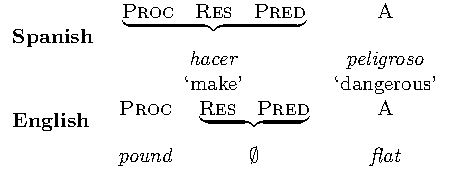
\includegraphics{lexicalization_table}}

Note that this account is consistent with the LPH because the variation is lexical in nature.
It is not immediately clear, however, that this lexical parameter could be learned from the primary linguistic data.
Since the head in question is phonologically null, there is, by definition, no direct evidence for it in (\textit{e.g.}) English. 
Therefore, the null head would have to be acquired indirectly, but \textcite{son2008microparameters} provide no proposals for how that would be done.
Absent any proposed method for acquiring this parameter, I will set it aside.
This means I will also set aside the structural analysis that is associated with the parameter. 

The final analysis I will address is that of \textcite{kratzer2004building}, which will not be fully rejected, but rather adapted to form my proposed structure.
In this analysis, the resultative object (\textit{e.g.}, \textit{the metal}) and the adjective (\textit{e.g.}, \textit{flat}) form a small clause, which describes a state.
The small clause merges with a \textit{res} head, which encodes a causative relation between events, and the resulting \textit{res}P is merged as the complement of the verb (\textit{e.g.}, \textit{hammer}).
The small clause theme is then raised to check accusative Case, and from there the derivation proceeds as normal.
The structure this generates is given in \Next.
\ex. Kratzer's Resultative Structure\\
{\small
\begin{forest}
  nice empty nodes,sn edges,baseline
  [AgrOP
  [{the metal},name=V theme]
  [
	  [AgrO]
    [VP
	[hammer] 
	[\textit{res}P 
	  [\textit{res}] 
	  [SC
	    [{$\langle\text{the metal}\rangle$},name=sc theme]
	    [flat]
	  ]
	]
      ]
    ]
  ]
  \draw[->] (sc theme) to[out=south west, in=south] (V theme);
\end{forest}}

Under the assumption that \textit{the metal} is $\theta$-marked by \textit{hammer}, this violates UTAH, and ought to be rejected.

\subsection{Summary}
In this chapter, I assessed several previous structural and parametric analyses of resultatives according to criteria I developed.
The structures proposed for resultatives were assesed in terms of UTAH, while the parameters proposed were assessed based on whether they could be learned from the primary linguistic data, and whether they were be represented as lexical parameters.
Several analyses were considered and ultimately rejected for not meeting the criteria I proposed.
However, Kratzer's (\citeyear{kratzer2004building}) structural analysis, and Snyder's (\citeyear{snyder1995language,snyder2012parameter}) parametric analysis appear to be promising, for reasons that will be further developed to form the analyses assumed in this thesis.

While portions of Snyder's and Kratzer's analyses were rejected, they share a certain feature which I will retain in my final analysis: they are acquirable.
Snyder's (\citeyear{snyder1995language}) proposal is that the availability of resultatives in a language is linked to the availability of a productive N-N compounding in that language.
Kratzer adopts this link and augments it with a link to predicative adjective agreement.
She proposes that resultatives (and N-N compounding) are available only in those languages in which predicative adjectives do not show agreement with the subject.
\ex. \textbf{German}
\ag. Die Teekanne leer trinken.\\
the teapot empty drink.\\
``to dring the teapot dry'' \parencite{kratzer2004building}
\b. Wurmkanne\\
``worm+can'' \parencite{snyder2001nature}
\cg. Die Teekanne ist leer (*-e).\\
The.\textsc{fem} teapot is empty \textsc{fem}''\\
``The teapot is empty.''

\ex. \textbf{Serbo-Croatian}\footnote{These examples are due to Mia Sara Misic (personal communication)} 
\ag.* Dario je ofarbao kucu crveno\\
Dario \textsc{cop} painted house red.\textsc{fem}\\
``Dario painted the house red.''
\b.* crve konzerva\\
``worm+can''
\cg. Ku\'ca je crven *(-a)\\
house \textsc{cop} red \textsc{fem}\\
``The house is red.''

Both compounding and the lack of predicative adjective agreement are detectable in the primary linguistic data, and therefore could reasonably be taken to be the positive data responsible for the setting of the resultative parameter.
The account of the resultative parameter which I will develop in the remainder of this thesis will build on the idea that the positive evidence that triggers the parameter setting will be related to compounding and adjectival agreement.
Before developing such an account, I will modify Kratzer's analysis to make it theoretically feasible in the next chapter.
\end{document}

